\section{Classical Algorithms: Description and Hyperparameters}
% ─────────────────────────────────────────────────────────────

\subsection{Evaluation Strategy: CV for Selection, Fixed Split for Reporting}

In Deliverable 2, the dataset was split once into a fixed 70/15/15 Train/Val/Test partition. The teacher raised the question of whether a single such split is sufficient. For the purposes of \textbf{hyperparameter selection}, this deliverable introduces \textbf{3-fold Stratified Cross-Validation} (CV), which generates three independent train/validation folds from the training subsample. Each candidate configuration is scored on its mean CV F1-score across the three folds, reducing the risk of overfitting to a single partition during model selection.

Critically, the \textbf{final evaluation} of each model—both baseline and best-tuned—is performed on the same held-out Test set used in Deliverable 2. This two-phase design answers the teacher's concern: CV provides statistical robustness during the search phase, while the fixed test set ensures results are directly comparable across deliverables and are not contaminated by the search process.

\subsection{Isolation Forest}

\textbf{Operating Principle.}
Isolation Forest \cite{liu2008isolation} builds an ensemble of $T$ isolation trees. Each tree is grown by recursively selecting a random feature $q$ and a random split value $p$ uniformly at random from $[\min(q), \max(q)]$. Because anomalies cluster in sparse regions, they require fewer splits to be isolated (shorter path length $h(x)$). The anomaly score is:

\begin{equation}
  s(x, n) = 2^{-\frac{\mathbb{E}[h(x)]}{c(n)}},
  \quad c(n) = 2H(n-1) - \frac{2(n-1)}{n}
\end{equation}

where $H(i)$ is the $i$-th harmonic number and $c(n)$ normalises for sample size $n$. A score near 1 indicates an anomaly; near 0.5 indicates a normal point.

\textbf{Key Hyperparameters Varied.}
\begin{itemize}
  \item \texttt{n\_estimators} $\in \{50, 100, 200\}$: number of isolation trees. More trees reduce variance but increase memory.
  \item \texttt{contamination} $\in \{0.10, 0.15, 0.20, 0.25\}$: expected fraction of anomalies, controls the decision threshold.
  \item \texttt{max\_features} $\in \{0.5, 0.75, 1.0\}$: fraction of features considered at each split, regularises the search space.
\end{itemize}

\textbf{Tuning Results.}
Figure~\ref{fig:if_heatmap} shows the mean CV F1-score across the full $3 \times 4 \times 3 = 36$-candidate grid. The best configuration (\texttt{n\_estimators=200}, \texttt{contamination=0.25}, \texttt{max\_features=1.0}) achieves a test F1 of 0.345, representing a gain of $+5.6$ percentage points over the default baseline (\texttt{n\_estimators=100}, \texttt{contamination=0.20}, test F1 = 0.289).

\begin{figure}[ht]
  \centering
  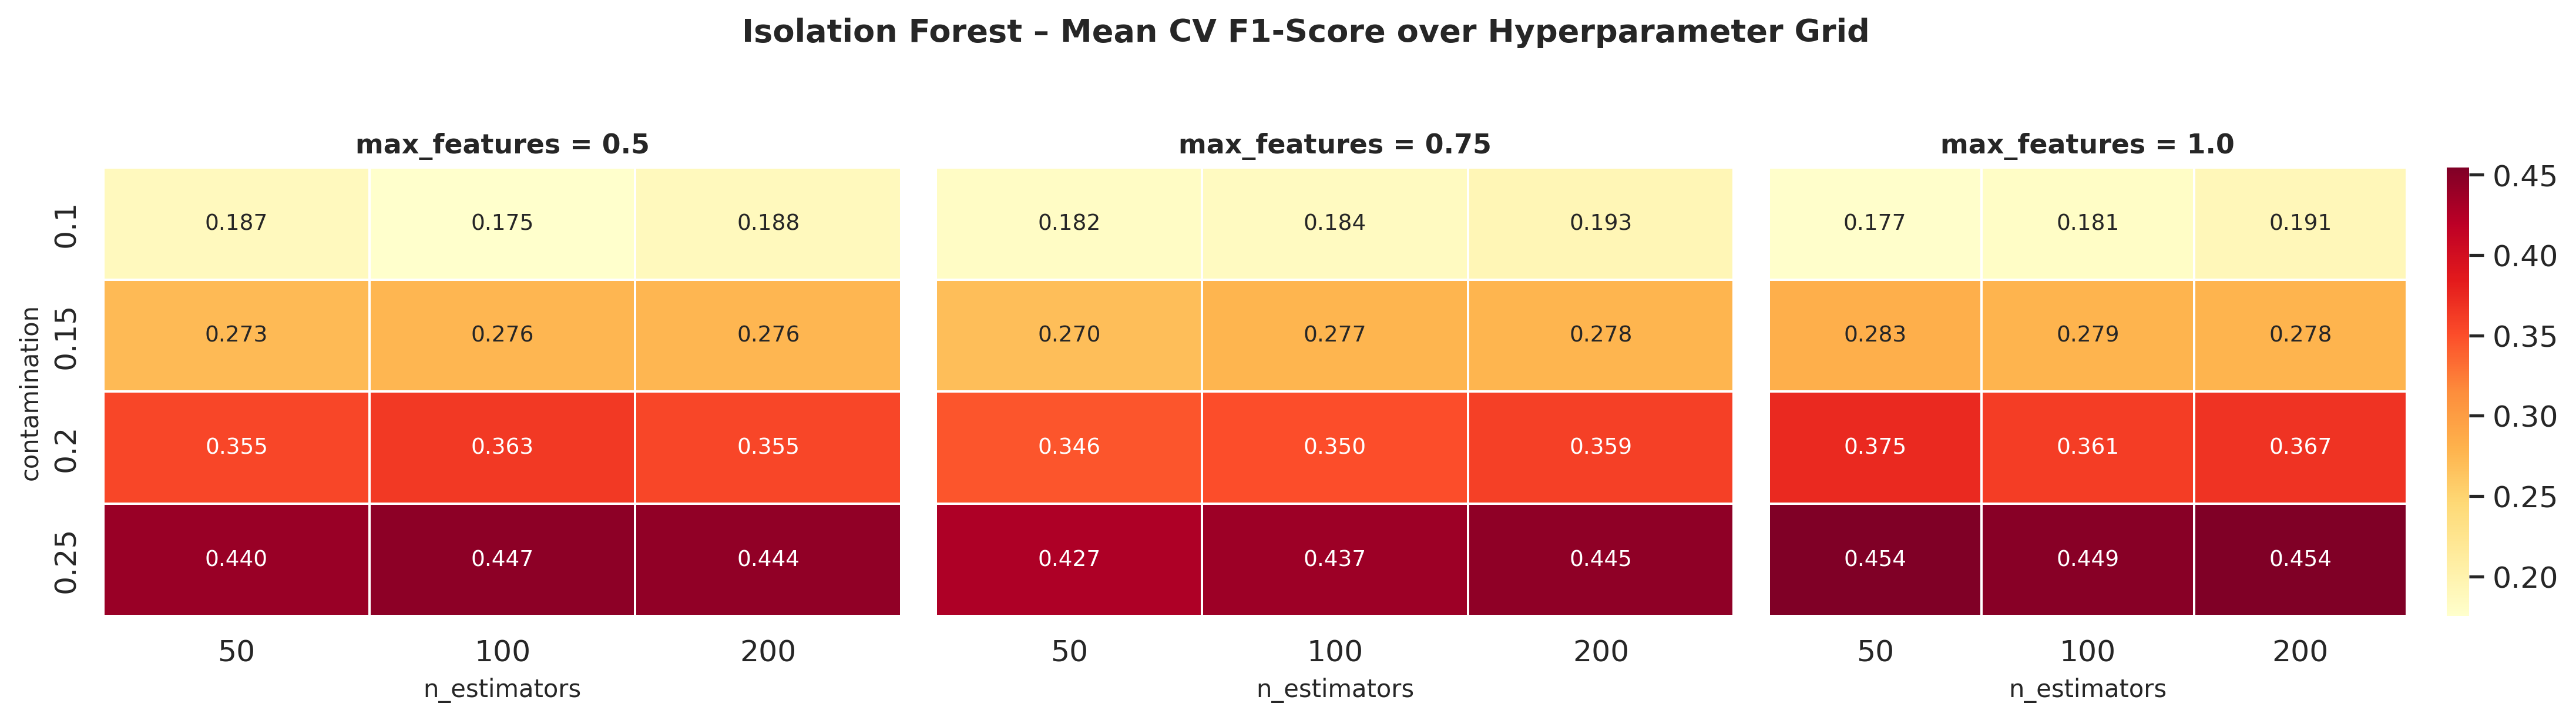
\includegraphics[width=0.48\columnwidth]{../tuning_results/if_heatmap.png}
  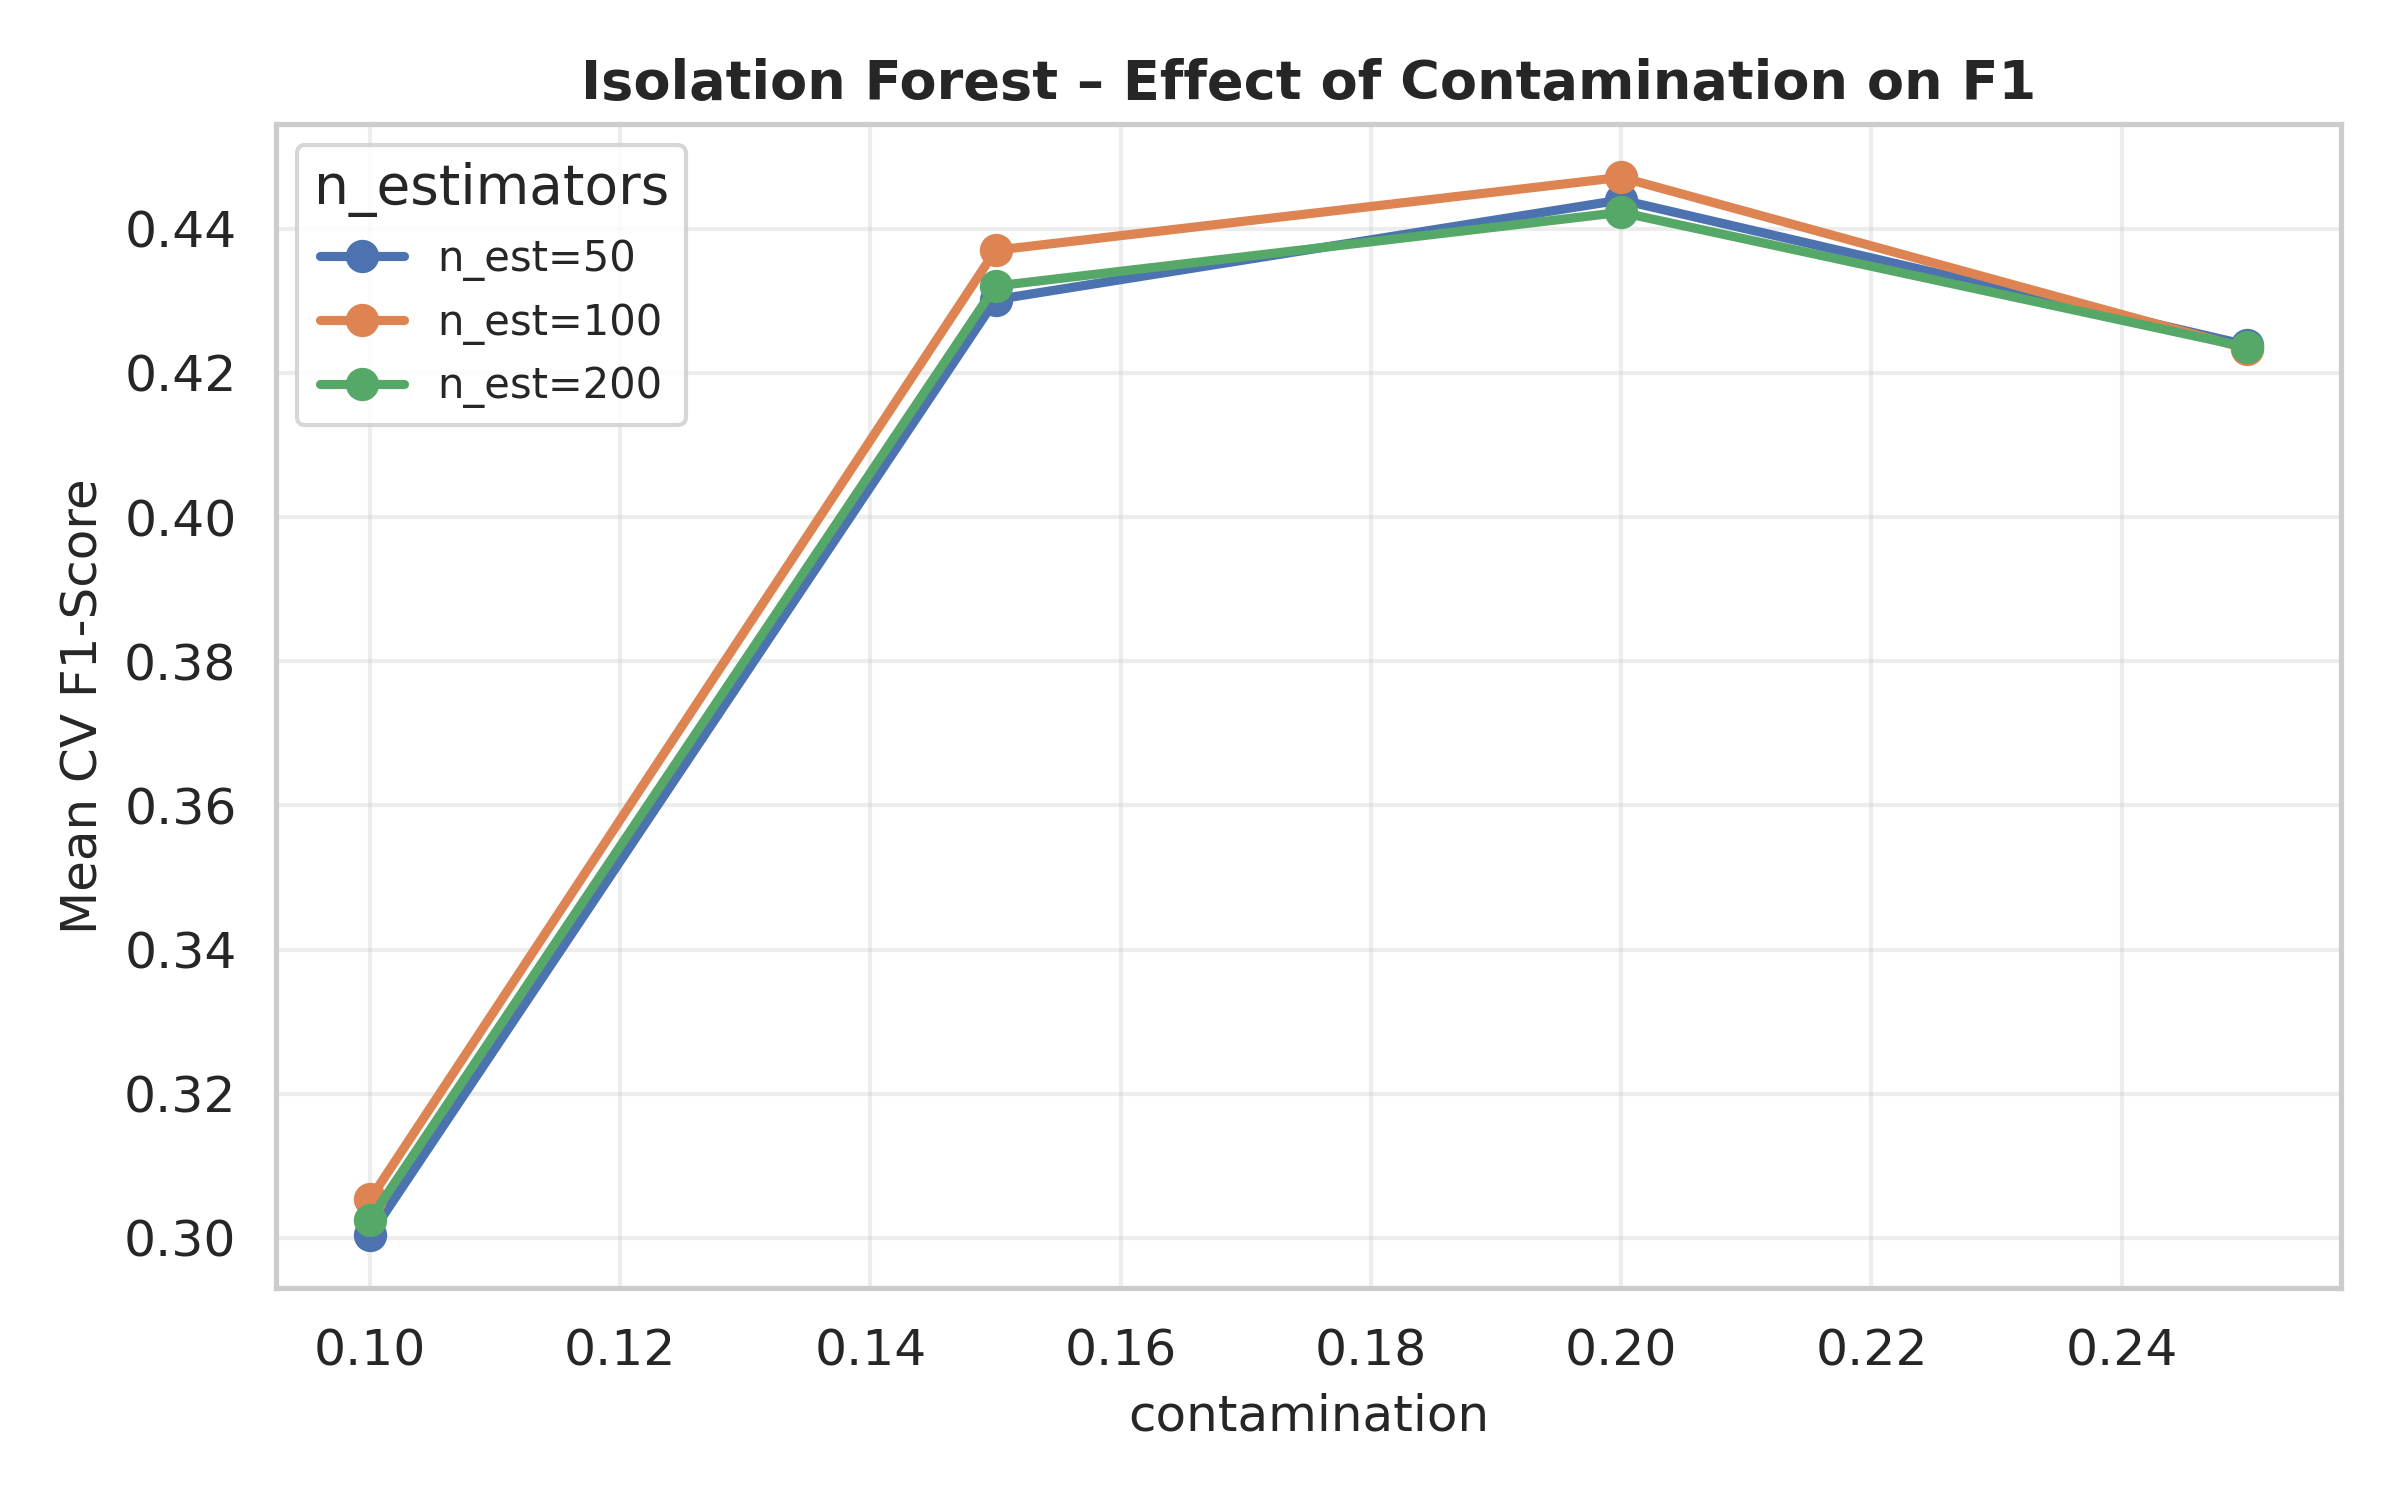
\includegraphics[width=0.48\columnwidth]{../tuning_results/if_contamination_effect.png}
  \caption{Left: IF mean CV F1 heatmap (contamination × n\_estimators).
           Right: Effect of contamination on F1 per n\_estimators.}
  \label{fig:if_heatmap}
\end{figure}

\subsection{One-Class SVM}

\textbf{Operating Principle.}
One-Class SVM \cite{scholkopf2001ocsvm} maps $n$ training points $\mathbf{x}_i$ through a kernel function $\phi$ into a reproducing kernel Hilbert space and finds the maximum-margin hyperplane $\langle \mathbf{w}, \phi(\mathbf{x}) \rangle = \rho$ separating the data from the origin:

\begin{equation}
  \min_{\mathbf{w},\rho,\boldsymbol{\xi}} \frac{1}{2}\|\mathbf{w}\|^2 - \rho
  + \frac{1}{\nu n} \sum_i \xi_i, \quad \xi_i \geq 0
\end{equation}

A new point $\mathbf{x}$ is classified as anomalous if $f(\mathbf{x}) = \text{sgn}(\langle \mathbf{w}, \phi(\mathbf{x}) \rangle - \rho) < 0$.

\textbf{Key Hyperparameters Varied.}
\begin{itemize}
  \item \texttt{kernel} $\in \{\text{rbf}, \text{poly}\}$: the RBF kernel captures non-linear manifolds of normal traffic; polynomial may generalise better in structured feature spaces.
  \item \texttt{nu} $\in \{0.05, 0.10, 0.15, 0.20, 0.25\}$: upper bound on the training-error fraction (anomaly rate prior).
  \item \texttt{gamma} $\in \{\text{scale}, \text{auto}\}$: RBF bandwidth, computed as $1/(n_\text{features} \cdot \sigma^2)$ for \texttt{scale} or $1/n_\text{features}$ for \texttt{auto}.
\end{itemize}

\textbf{Tuning Results.}
Figure~\ref{fig:ocsvm_heatmap} shows that the RBF kernel consistently outperforms polynomial for this dataset. The best configuration (\texttt{kernel=rbf}, \texttt{nu=0.25}, \texttt{gamma=scale}) achieves a test F1 of 0.273 vs.~the baseline 0.243 ($+3.0$~pp). Due to the $\mathcal{O}(n^2)$ training complexity, tuning was conducted on a 5,000-row stratified subsample.

\begin{figure}[ht]
  \centering
  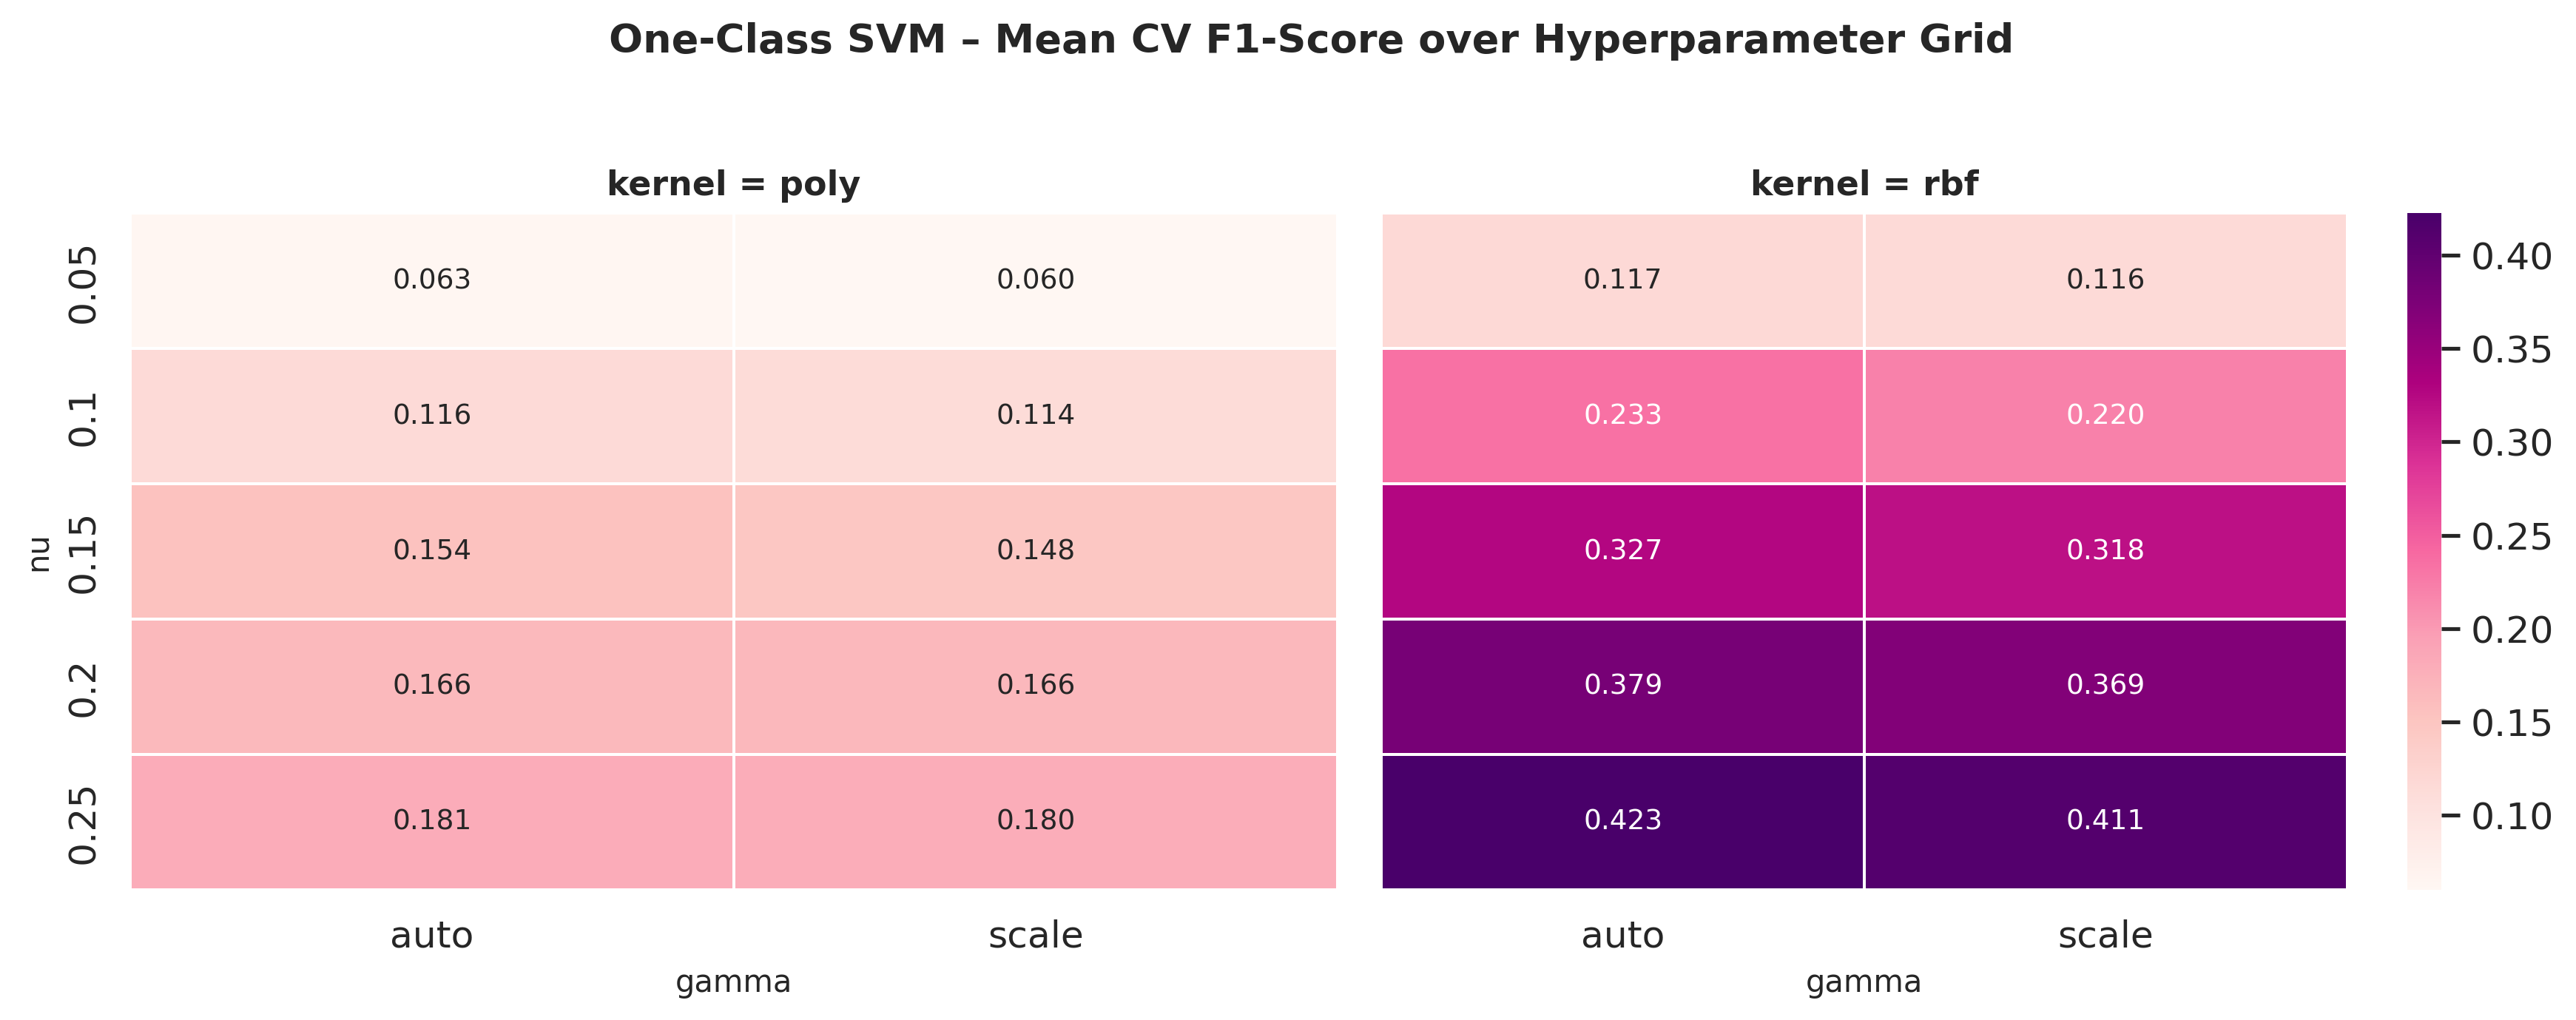
\includegraphics[width=0.58\columnwidth]{../tuning_results/ocsvm_heatmap.png}
  \caption{OC-SVM mean CV F1-Score heatmap (nu × gamma per kernel).}
  \label{fig:ocsvm_heatmap}
\end{figure}

\subsection{Local Outlier Factor}

\textbf{Operating Principle.}
LOF \cite{breunig2000lof} computes a local density estimate for each point $p$ based on the $k$-nearest-neighbour \emph{reachability distance}:

\begin{equation}
  \text{lrd}_k(p) = \frac{k}{\sum_{o \in N_k(p)} \text{reach-dist}_k(p, o)},
  \quad
  \text{LOF}_k(p) = \frac{\sum_{o \in N_k(p)} \frac{\text{lrd}_k(o)}{\text{lrd}_k(p)}}{k}
\end{equation}

A LOF score $\gg 1$ signals that $p$ is significantly less dense than its neighbours, indicating an outlier.

\textbf{Key Hyperparameters Varied.}
\begin{itemize}
  \item \texttt{n\_neighbors} $\in \{5, 10, 20, 40, 60\}$: the neighbourhood size $k$. Larger $k$ smooths density estimates but can miss local outliers.
  \item \texttt{contamination} $\in \{0.10, 0.15, 0.20, 0.25\}$: threshold for the decision boundary.
\end{itemize}

\textbf{Tuning Results.}
As shown in Figure~\ref{fig:lof_heatmap}, LOF is the most sensitive of the three models to hyperparameter choice, yet its overall CV F1 remains below 0.20 regardless of configuration. This confirms the theoretical expectation: LOF's density-ratio approach degrades severely in the 70-dimensional feature space due to distance concentration \cite{zimek2012survey}.

\begin{figure}[ht]
  \centering
  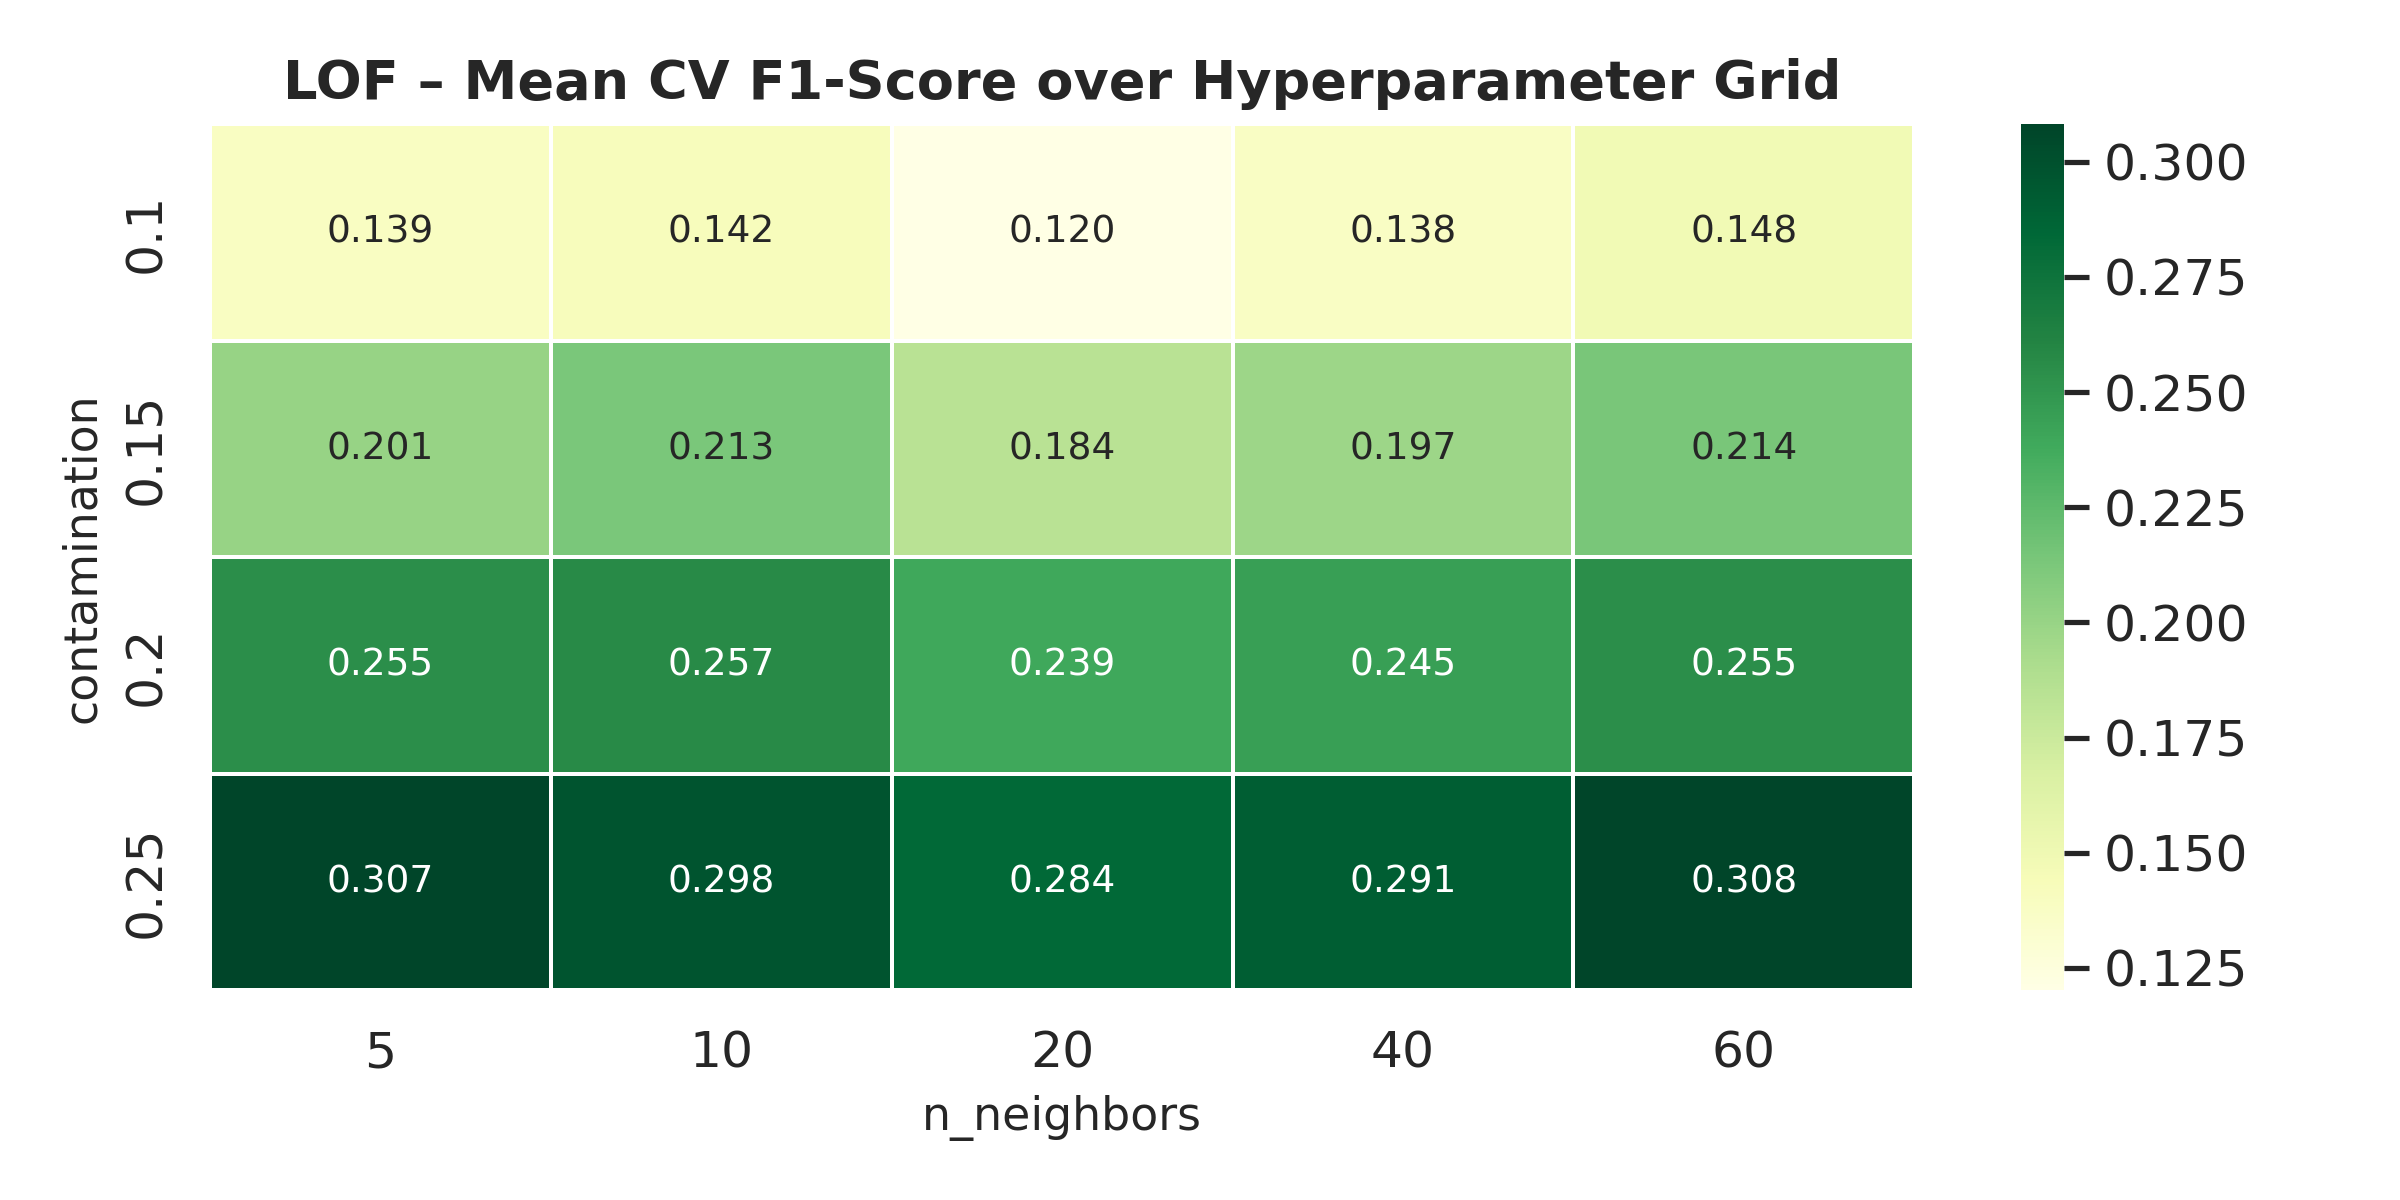
\includegraphics[width=0.48\columnwidth]{../tuning_results/lof_heatmap.png}
  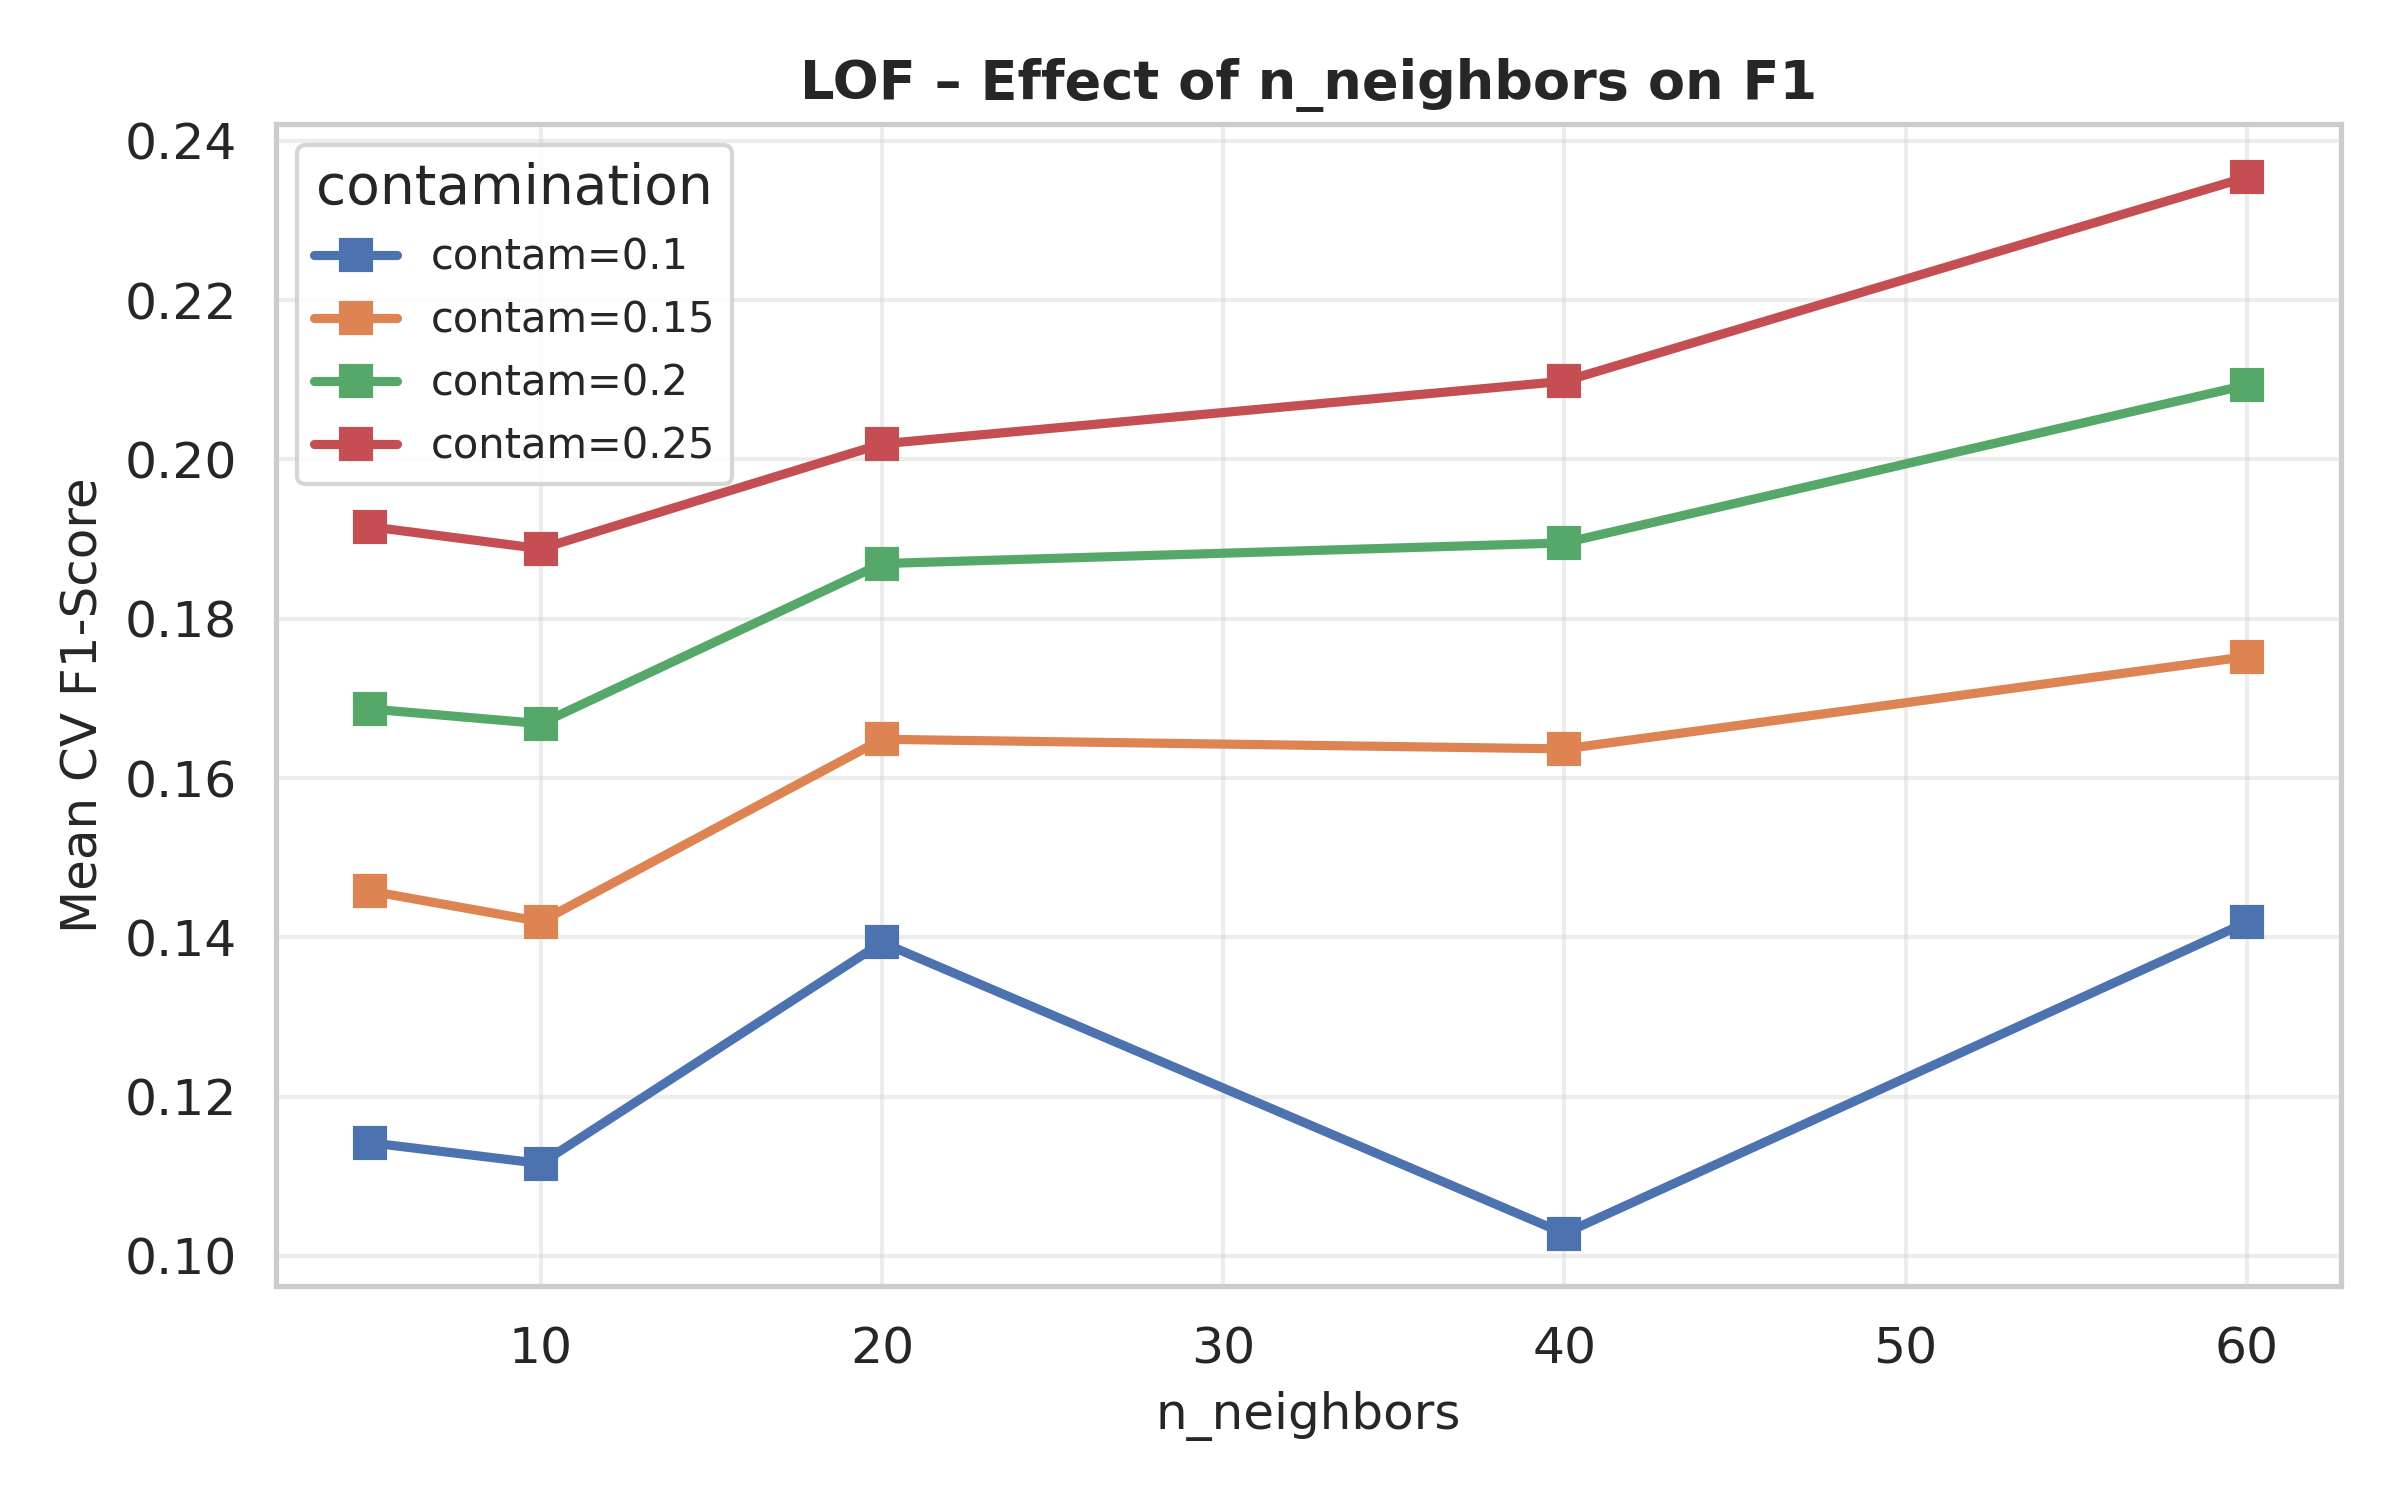
\includegraphics[width=0.48\columnwidth]{../tuning_results/lof_neighbors_effect.png}
  \caption{Left: LOF CV F1 heatmap (contamination × n\_neighbors).
           Right: Effect of n\_neighbors on F1 per contamination.}
  \label{fig:lof_heatmap}
\end{figure}

\subsection{Baseline vs.\ Tuned Performance}

Figure~\ref{fig:baseline_vs_best} compares the default-parameter baseline against the best-found configuration for each model, evaluated on the held-out Test set. Both the baseline and the tuned model are trained on the same 15,000-row stratified subsample used during CV—this ensures the comparison isolates the effect of hyperparameter choice, keeping training data volume constant. Note that these absolute F1 values are therefore lower than the full-data results reported in Deliverable 2 (where Isolation Forest was trained on $\approx$395,000 rows); what matters here is the \emph{delta} between baseline and tuned configurations within the same experimental conditions.

Isolation Forest benefits most from tuning ($+5.6$~pp F1: 0.289~$\to$~0.345), OC-SVM gains modestly ($+3.0$~pp: 0.243~$\to$~0.273), and LOF shows negligible improvement ($+0.8$~pp: 0.174~$\to$~0.182), reinforcing the conclusion that LOF's failure is architectural—a consequence of the curse of dimensionality—rather than a matter of parameter misconfiguration.

\begin{figure}[ht]
  \centering
  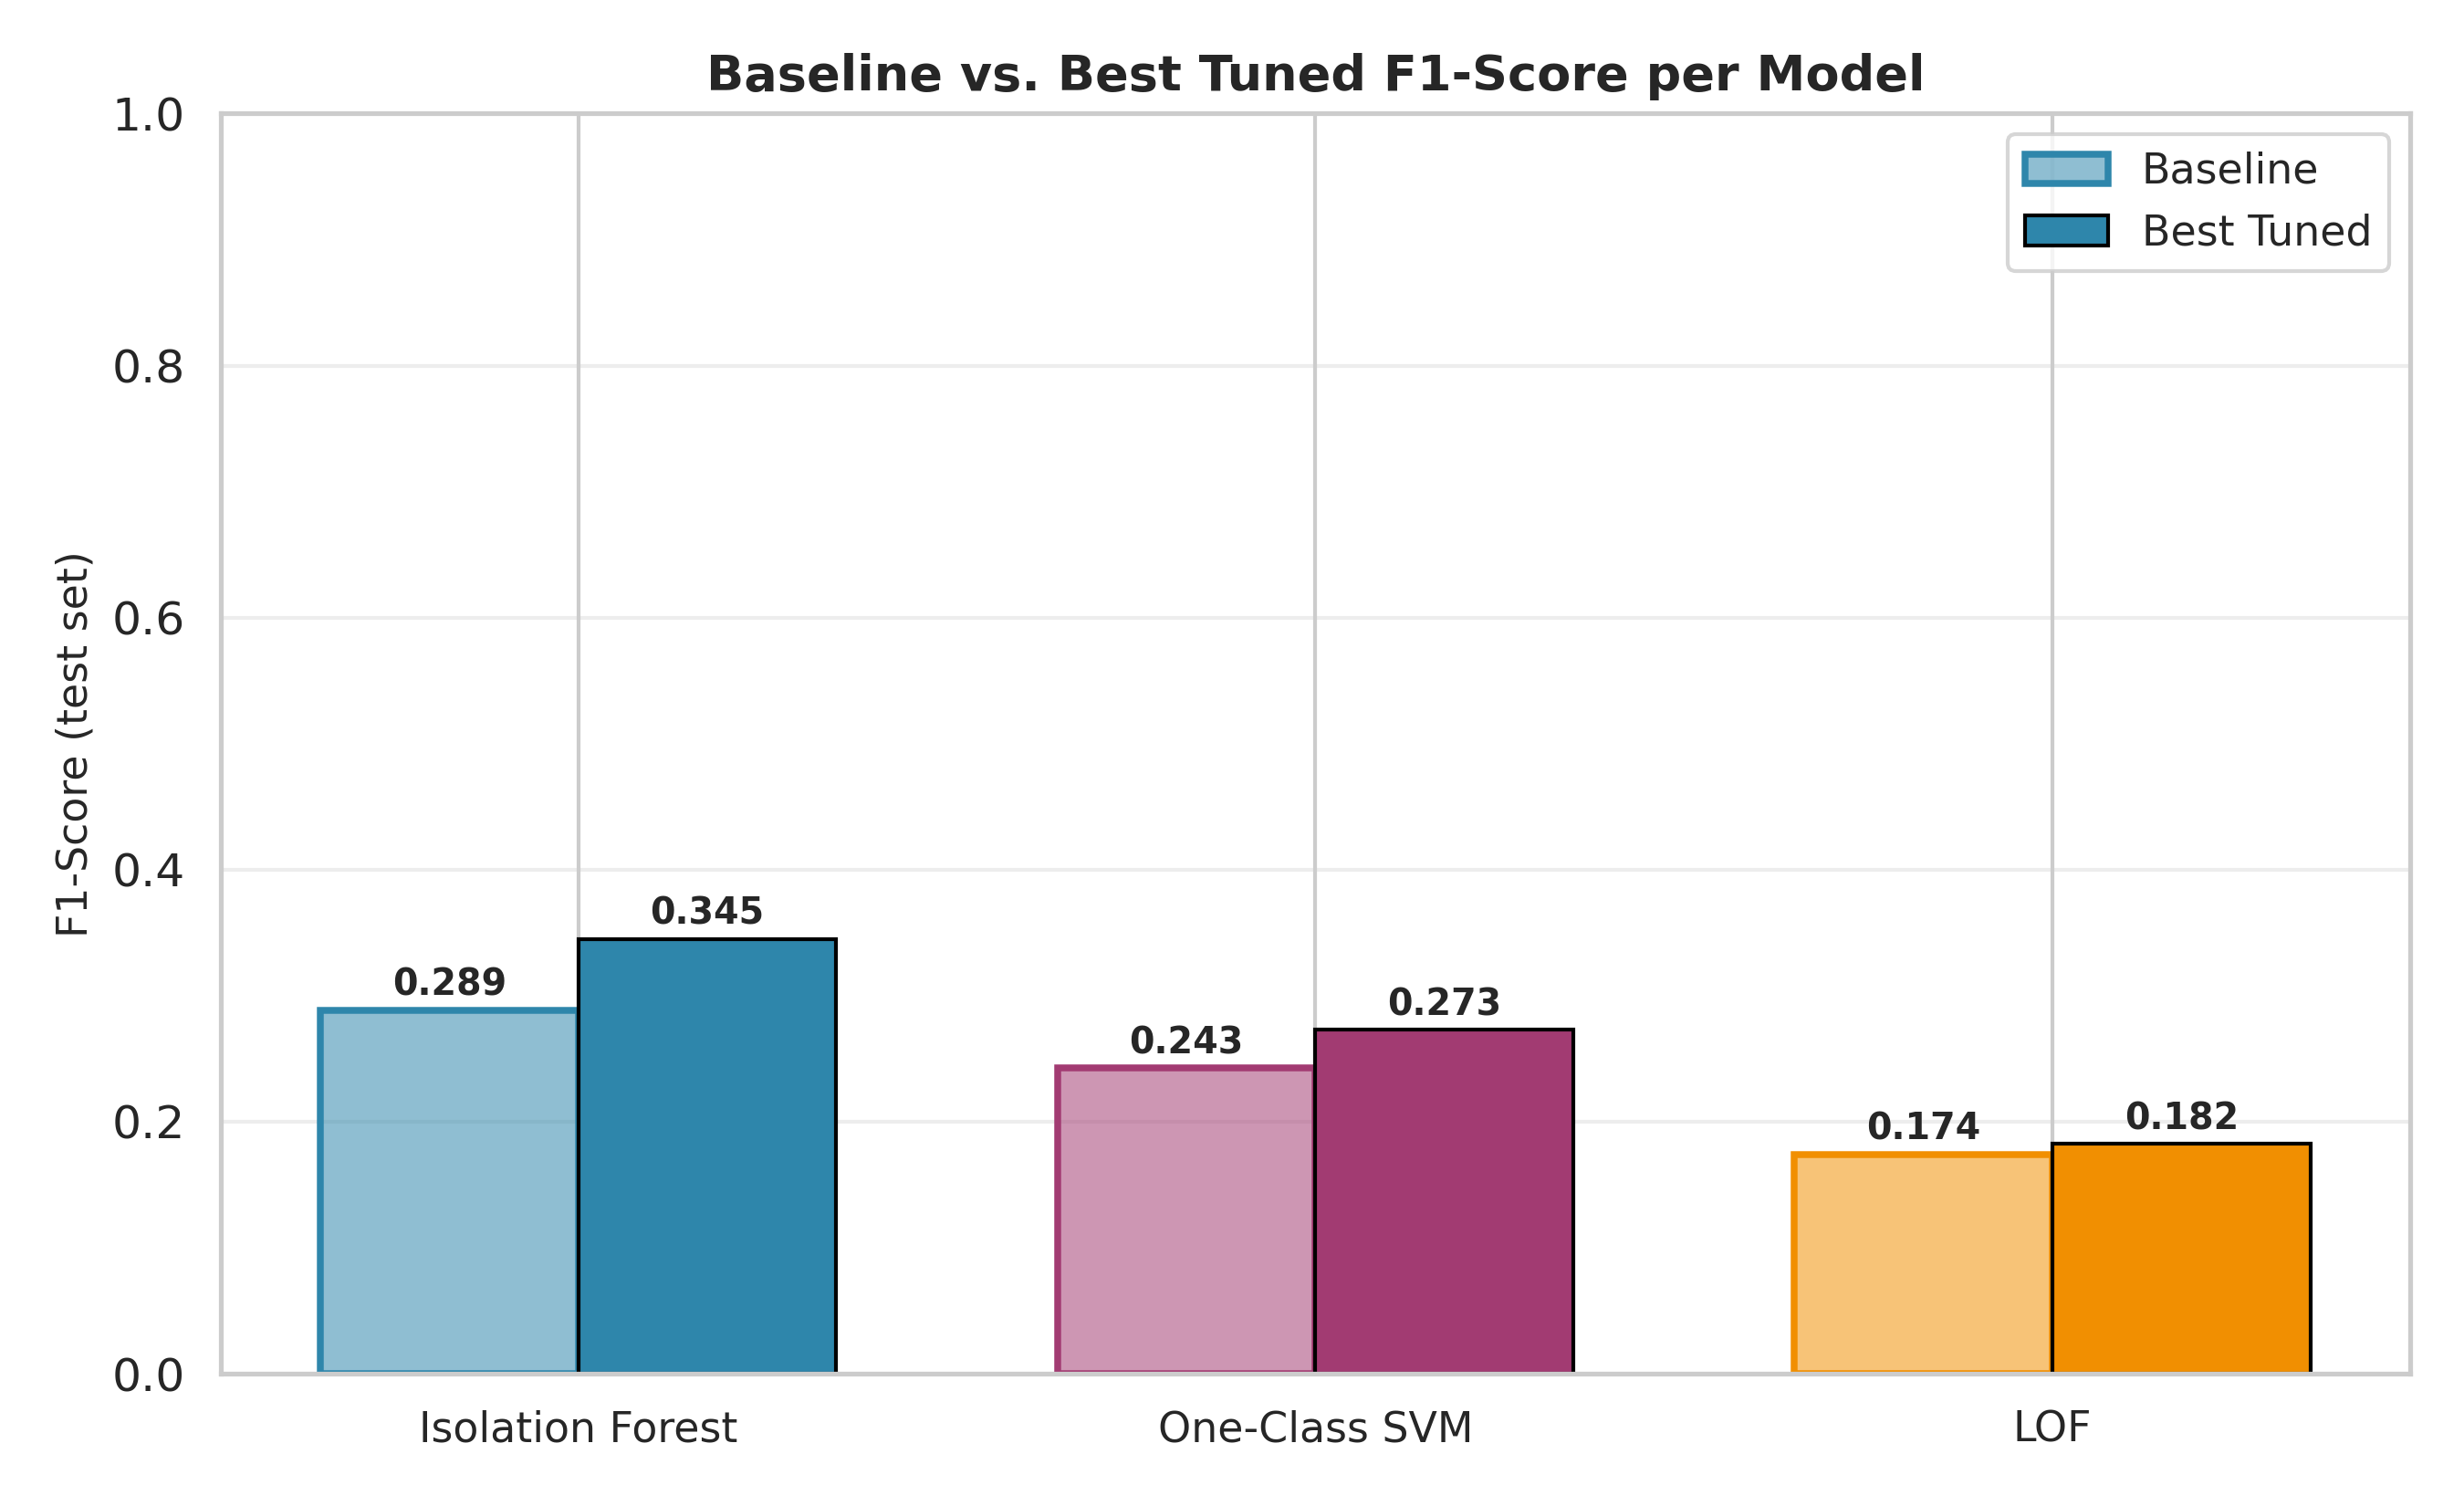
\includegraphics[width=0.58\columnwidth]{../tuning_results/baseline_vs_best.png}
  \caption{Test-set F1-Score: default baseline vs.\ best hyperparameter configuration.}
  \label{fig:baseline_vs_best}
\end{figure}

% ─────────────────────────────────────────────────────────────
